\documentclass[letterpaper]{article}
%\usepackage{times}
%\usepackage{helvet}
%\usepackage{courier}
\usepackage{cite}
\usepackage{amsmath}
\usepackage{amsthm}
\usepackage{graphicx}
\usepackage{fancyhdr}
\usepackage[bottom]{footmisc}
\usepackage{amssymb}
\usepackage{enumerate}
\usepackage{mathtools}
\usepackage{array}
\usepackage{color}
% algorithms
\usepackage{algorithm}
\usepackage[noend]{algpseudocode}

%===================================
% margins
\usepackage{geometry}
%\geometry{
%	letterpaper,
%	right=20mm,
%	left=20mm,
%	top=10mm,
%	bottom=20mm
%}
\usepackage[pdftex,
 pdfauthor=Soheil Gharatappeh,
 pdftitle={Apprenticeship Learning Approach to Inverse Reinforcement Learning},
 pdfsubject={Sample document with blind text},
 pdfkeywords={hyperref, PDF meta information},
 pdfproducer=TeXShop,
 pdfcreator=pdflatex]{hyperref}

%============ FUNCTIONS =============
\newcommand{\valatrisk}[2]{\operatorname{VaR}_{#1}(#2)}
\newcommand{\cvalatrisk}[2]{\operatorname{CVaR}_{#1}(#2)}
\newcommand{\norm}[2]{{\Vert{#1}\Vert}_{#2}}

\newenvironment{mprog}{\begin{array}{>{\displaystyle}l>{\displaystyle}l>{\displaystyle}l}}{\end{array}}
\newcommand{\cs}{\\[1ex] & }
\newcommand{\stc}{\\[1ex] \mbox{s.t.} &}
\newcommand{\minimize}[1]{\min_{#1} &}
\newcommand{\maximize}[1]{\max_{#1} &}

\newcommand{\tr}{^{\mathsf{T}}}
\newcommand{\zero}{\mathbf{0}}
\newcommand{\st}{\quad\text{s.t.}\quad}
%===================================

\newcommand{\eye}{\mathbf{I}}
\newcommand{\one}{\mathbf{1}}
\newcommand{\marek}[1]{\textcolor{red}{[#1]}}

\frenchspacing
\setlength{\pdfpagewidth}{8.5in}
\setlength{\pdfpageheight}{11in}
\pdfinfo{
/Title (Predicting Death In Game of Thrones)
/Author (Soheil Gharatappeh)}
\setcounter{secnumdepth}{0}  

\title{Predicting Death In Game of Thrones}
\author{Soheil Gharatappeh}

\begin{document}
\maketitle
	
	
% \begin{abstract}
% \begin{quote}

% \end{quote}
% \end{abstract}

\section{Introduction}
These days Machine Learning tools are being widely used to predict different phenomenas. From the stock market, to autonomous cars, researchers are interested to have their prediction on all aspects of life. Recently, the movie Game of Thrones has gained a huge popularity, and everyone was wondering \textit{which of the characters can make it to the end?}. This could be a great subject for a research project in Data Science realm. There are various resources of information, from structured wikis to un-structured text such as the books of this legend. We can base our prediction on information that is coming from all of these resources. However, using the right information helps to put all pieces of this puzzle together.


One rich and valuable piece of information we have access to is a data set obtained by the fan's community. This data set contains various information, from the date of birth, to the allegiances, nobility, gender, etc., and can be used to train different machine learning methods, in order to find out what aspects of the information is the most influential in the chance of death for each character.


For the next phase in the project, we would like to omit the data set, and work only with the wiki and un-structured text of the books. This means the project will shift from a purely machine learning project, towards a more realistic practical data science one, where we need to obtain the information we need, clean it, filter it, and then use that information as a single feature for the machine learning algorithm. Obtaining information from un-structured text is very hard, due to the noisy and nonlinear nature of natural language. 


In order to tackle this issue, we can use knowledge bases. A knowledge base is a big set of triple entities (two names connected with a relation), obtained from a structured text such as wiki, and contains rich information about the world's entities, their meanings, and relationships. Knowledge bases give structure to the raw and noisy data obtained from the web, and makes them usable for a machine. A crucial part of this process is entity linking, where a named entity is linked to the knowledge base.


This work is heavily based on the idea of entity linking and knowledge graphs. In the following sections, we first introduce entity linking and review a few related works in this area. Then, we explain our approach to the problem of using entity linking in order to predict the chance of death for a GoT character, and at the end, we evaluate our work using different measures.

\section{Background}

Knowledge sharing platforms such as Wikipedia, play an important role in creating machine-readable knowledge bases. Knowledge bases contain rich information about the world's entity, and their relationships. Using KB's, one can extract useful information from the raw and noisy data in a text. Entity linking is a key element of this process, where a named entity is linked to the knowledge base.

The entity linking is a challenging task. Name variations, aliases, abbreviations, alternate spellings result in entity ambiguity. The task is to find a map from between a set of pre-identified textual entity mentions m into their corresponding entity in the knowledge base. There, also, might be some entities in the text with no entity record in the knowledge base (unlinkables or NILs).

The process starts with name entity recognition, where the boundaries of the entity is identified. There are three steps in the task of entity linking; candidate entity generation, candidate entity ranking, and unlinkable mention prediction. In the first step, a relevant subset of entities are retrieved from the knowledge base. Then, we need to rank them in the next step, so that we know which node in the knowledge base is more relevant to our entity and which one is less relevant. And, at the end, we need to have a strategy to deal with unlinkables \cite{entity}.


In order to evaluate each of these algorithms, a few metrics have been introduced in \cite{entity}, such as precision, recall, accuracy, and F1-score. Also, some data sets are published in \cite{entity} in order to be used as the ground truth for this field. Going through the list of all available data sets is out of the scope of this writing.

 
In another related work, Cheng et at. introduced Relational Inference for Wikification \cite{cheng-2013}, where they are trying to disambiguate entities in a text by identifying the context of it, and relating an entity to the most relevant Wikipedia page. The idea is to use the relational structure of the text in order to generate more relevant title candidates, rank them better and deal with unlinkables more efficiently. They form an Integer Linear Program using the document and the knowledge base consist of triples, and solve it to find the best assignment for each title-surface set (where surface is an entity mention). This approach is evaluated in comparison to other Wikification systems such as Milne and Witten (M\&W), and Ratinov et al. (R\&R) by using data sets from GLOW system, a work by Ratinov et al. and evaluating it with Bag of Titles (BOT) F1 measure. The results suggest a good level of improvement over all 4 different data sets, in comparison with M\&W and R\&R. They also compared their approach to top 3 TAC 2011 systems, where they used $B^3$ and Micro-Average as the evaluation metric. Their system performed comparatively similar to the top 3.


Also, in \cite{tagme}, Ferragina et al. talk about adding Wikipedia links to the respective mentions of entities in a text. The contribution of this method is its applicability to short or poorly composed texts, such as tweets, snippets of search engines, etc. The idea is to use Wikipedia anchor texts as spots and pages that are linked to them as a possible meaning for each entity. The ambiguity is solved by using a fast and effective scoring function, which exploits the sparseness of the anchors in a short text. One important phase in disambiguation is prunning un-meaningful anchors by using the link probability and coherence of a candidate annotation. This approach is evaluated in comparison Milne \& Witten method on three different data sets, the first one is derived manually, and the second and the third is from Wikipedia. They evaluating their method with F measure, precision and recall. The results show that tagme outperformed in short texts, and have a good comparative performance on long texts in compared with Milne \& Witten method.


In \cite{dbpedia}, Mendes et at. explain their approach to automating the process of text document annotation with DBpedia URIs. The goal is to find and disambiguate DBpedia mentions automatically and adaptively, for the needs of each user, specifically. The idea is, to recognize the entity in a sentence, first. Then,to map the entity to a selection of candidates from DBpedia. Next, using the context around the entity, the disambiguation stage is proceed. And, at the end, we let the user to customize the resulted annotation for his need through the configuration parameters. They evaluated their disambiguation strategy on some unseen DBpedia resource mentions from Wikipedia. They used accuracy for evaluating their system, and it suggests a good upgrade in compared to all baseline methods. But, unfortunately, they didn't provide any accuracy results for other publicly available approaches, and they only compared their algorithm with those methods in terms of precision-recall paradigm. They also tested their system on a set of manually annotated news article, and compared their annotation with other publicly available annotation systems. They evaluate their algorithm using F1 measure and compared it to other methods. But, as the result suggested, they could not outperform the wiki machine. But, they did better than the others in terms of F1 score.


\section{Approaches} \label{sec:approach}

\subsection{Entity Linking}

In this section, the approaches for tackling the problem of predicting the death of a GoT character is explained. One of the main ideas, were to first train a perfect classifier using the data set, and then discard the features that are read from the prepared data set, and extract those features purely from the books. Although the idea seemed appealing and sound at the beginning, it had a big flaw, and that was; extracting features from an unstructured text is a drastically hard task, if not even impossible. This is where having a knowledge base, and doing entity linking over it can be helpful. Using a knowledge base (that is obtained, for example, from the GoT's Wiki), we can employ entity linking in order to disambiguate entities. Entity linking can be helpful in constructing a big feature vector for each entity (each attribute in the Wiki can be served as a feature), which can later on be used to train a classifier. The more accurate entity linker we use, the better result we get from the classifier.

However, having a complete knowledge base is essential in the procedure of entity linking. It is usually the case that because of having multiple entity in the knowledge base corresponding to the surface, we need to rank the entities so that we can retrieve the most relevant entity to the user. But, unfortunately, that is not the case in here. There is a limited number of wiki pages for each character, with a very limited information. Only 263 of characters of the data set have a corresponding node in the knowledge base. Therefore, I did not include the entity linker features into the set of features.

\subsection{Gender Prediction}

It is very important to determine which of features in the data set are the most useful ones. Factoring out the less informative feature eliminates noises from adding to the data and helps the classifier to gain a better accuracy. The problem of finding the best features is heavily tied with the problem of which features of the data set can be extracted from the knowledge base and the book with higher certainty. One can come up with a set of features coming out of a regularization method (such as lasso), with a high accuracy. But, if extracting those features from the text and the wiki is not feasible, then we have to eliminate that feature.


A gender classifier is implemented, which uses the pronouns to predict the gender of a character in the sentence. Two methods are tried for determining the gender. First, we use a pronoun counter to make the decision. We count the number of pronouns in the sentence that a name occurs and the sentence after, and the gender is obtained by the dominant pronoun. Second, we apply closeness measure to predict the gender, and we assign the gender of the closest pronoun to each corresponding noun. 


\subsection{Features}

Based on various experiments, we figured out that features such as the gender, the mention frequency, mention of the name in different sections of the book and how the mention count distributed among different books, and proximity of the character's name in the book to some deadly words are the most useful features. Therefore, we employ various tools to obtain a prediction from the above-mentioned features. To obtain the proximity of a character to deadly words, we first find the places in the books in which the character appeared in the same sentence with a deadly word (a hand-crafted list of words prepared for this matter which contains words like stab, kill, die, etc.). Then the tf-idf score of this sentences (deadly sentence) is calculated against a sentence containing all of the deadly word and the character's name. Then, this score is used as a feature to train the classifier.


% We also create different types of knowledge graphs using the knowledge base, by extracting different aspects of each character. For instance, in case of the gender predictor, we can use the information we have in a the wiki page of the character to extract the gender. We can use the idea of pronoun count in the wiki to predict the gender. Also, other informations from the knowledge base, such as the relation between characters can be used to create a graph and measure the centrality of each character, and the closeness of a character to more important figures.

Another problem to address in this project is disambiguation. A lot of names in the book are not fully written, and that makes them ambiguous. The way we currently define an entity mentions is if a) the name fully appears in a sentence b) one part of the name appears in a sentence. A tf-idf score of a wiki page against the sentence that this name occurred in can be used for disambiguating names in the book. But, for this submission, we only consider scenario b, where appearing one part of a name is enough for being considered as an entity occurrence.



% graphs

% approaches
%     entity linking and other methods,
%     gender classifier
%     preprocessing
%     features (can include the entity linking features in here)
%     ML/how to combine them




\section{Evaluation}

In this section, we explain the metrics we used to evaluate the project, and analyze the  obtained results. The metric we used to evaluate our approach is F1-score. In total we have five sets of features; 1) total mention count 2) mention count per book 3) gender (frequency of pronoun and closest pronoun) 4) number of occurrence with a deadly name at the same sentence 5) tf-idf of collection of deadly sentences. The following plot is F1-score of various classifiers using the same set of features.

As one can see in figure \ref{fig:f1}, KNN with $k=9$ has the best score. The $k$ value in KNN is selected based on another experiment, where $k=3,..., 12$ were tried, and $k=9$ had the best validation error.

It is worth mentioning that in the process of adding more features to the system, the f1-score for the best-performing method has changed from $0.6349$ with only count features to $0.6364$ by adding the gender, and to $0.6383$ when adding the deadly word proximity features.

\begin{figure}
	\centering
	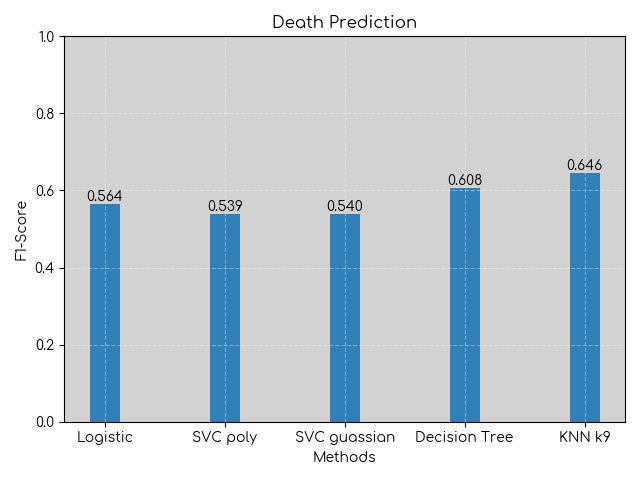
\includegraphics[scale=.60]{f1_scores.png}
	\caption{F1-score of various classifiers on a set of features completely obtained from the text.}
	\label{fig:f1}
\end{figure}

In another experiment, the rule-based gender classifier explained in section \nameref{sec:approach} trained and tested using the same set of data as the previous experiment. The result of this experiment is shown in figure \ref{fig:gender}

\begin{figure}
	\centering
	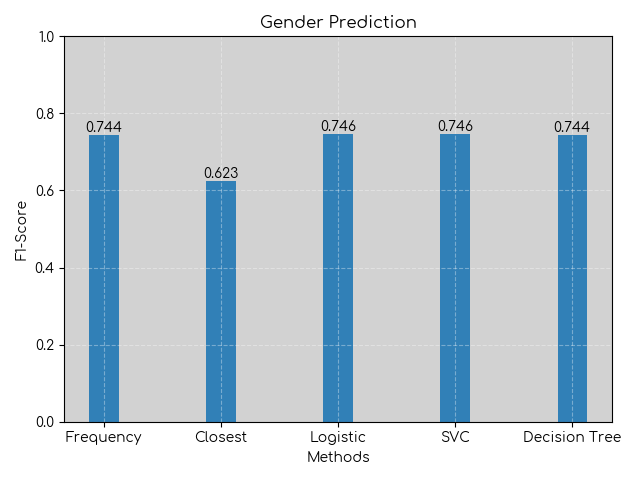
\includegraphics[scale=.60]{gender_prediction.png}
	\caption{F1-score of gender classifier. The first two bars are related to the rule-base predictor, and bar 3-5 are f1-score of different classifiers using those rule-base feature for training.}
	\label{fig:gender}
\end{figure}


results shouldn't be only some numbers, explain!
evaluation of the gender classifier





\section{Future Work}



\bibliographystyle{plain}
\bibliography{invasive_species}

\end{document}




%===============================
%========== NOT TO RUN =========
\iffalse

\begin{equation}\label{eq:lp_dual}
\begin{mprog}
\maximize{\mathbf{u}} \mathbf{u}\tr  \mathbf{r} 
\stc \sum_{a \in \mathcal{A}}(\mathbf{I} - \gamma \mathbf{P}_a)\tr\mathbf{u}_a = \mathbf{p}_0 
\cs \mathbf{u}_a \geq \mathbf{0}
\end{mprog}
\end{equation}


\usepackage{titlesec}

\titleformat{\section}
  {\normalfont\Large\bfseries}   % The style of the section title
  {}                             % a prefix
  {0pt}                          % How much space exists between the prefix and the title
  {Section \thesection:\quad}    % How the section is represented

% Starred variant
\titleformat{name=\section,numberless}
  {\normalfont\Large\bfseries}
  {}
  {0pt}
  {}
  

asdasd \cite{1013341}. Fig.~\ref{Fig_Example}.

{\fontfamily{pcr}\selectfont 
run files}

\begin{enumerate}
  \item The labels consists of sequential numbers.
  \item The numbers starts at 1 with every call to the enumerate environment.
\end{enumerate}

\begin{itemize}

\end{itemize}

======== HYPERLINK =============
Find the \texttt{run files} for all variants in \href{https://github.com/SHi-ON/InfoRet/tree/master/results/Assignment_4}{here}


====== FIGURES ========

\begin{figure}
	\centering
	\includegraphics[scale=.40]{Fig_Example.pdf}
	\caption{Example.}
	\label{Fig_Example}
\end{figure}

\input{second}

========= EQUATIONS =============

\begin{equation}
\left\|\frac{\partial V}{\partial\mathbf{x}_1}\right\|\left\|\mathbf{x}_1\right\|\leq c_1V\quad \text{for}\; \left\|\mathbf{x}_1\right\|\geq c_2
\end{equation}


============ TABLES =============

\begin{tabular}{ |p{3cm}|p{3cm}|p{3cm}|  }
\hline
\multicolumn{3}{|c|}{Country List} \\
\hline
Country Name     or Area Name& ISO ALPHA 2 Code &ISO ALPHA 3 \\
\hline
Afghanistan & AF &AFG \\
Aland Islands & AX   & ALA \\
Albania &AL & ALB \\
Algeria    &DZ & DZA \\
American Samoa & AS & ASM \\
Andorra & AD & AND   \\
Angola & AO & AGO \\
\hline
\end{tabular}

\begin{center}
\begin{tabular}{ |c|c|c| } 
 \hline
 cell1 & cell2 & cell3 \\ 
 cell4 & cell5 & cell6 \\ 
 cell7 & cell8 & cell9 \\ 
 \hline
\end{tabular}
\end{center}




\begin{lstlisting}[language=Python, caption=Code's name]
import numpy as np
 
def incmatrix(genl1,genl2):
    m = len(genl1)
    n = len(genl2)
    M = None #to become the incidence matrix
    VT = np.zeros((n*m,1), int)  #dummy variable
\end{lstlisting}



\begin{verbatim}
Put your codes here!
\end{verbatim}
\fi
